\documentclass[a4paper,14pt,russian]{extarticle}
\usepackage[utf8]{inputenc}
\usepackage[russianb]{babel}
\usepackage{vmargin} % set margins and
\usepackage{fancyhdr} % custom page numbering
\usepackage{setspace} % https://proft.me/2013/06/9/latex-ukazanie-mezhstrochnogo-intervala/
\usepackage{indentfirst}
\usepackage{float} % algo
\usepackage{amsmath}
\usepackage{amssymb}
\usepackage{amsthm}
\usepackage{amsfonts}
\usepackage{hyperref}
\usepackage{graphicx}
\usepackage[ruled]{algorithm2e}
\usepackage{caption}


\graphicspath{ {../figures/} }

% \usepackage{tikz} % charts
% \usepackage{pgfplots} %charts

\setmarginsrb{3.5cm}{2cm}{1cm}{2cm}{0pt}{0mm}{0pt}{0mm}
\linespread{1.3}
% header and footer
\pagestyle{fancy}
\fancyhead{}
\fancyfoot{}
\renewcommand{\headrulewidth}{0pt}
\renewcommand{\footrulewidth}{0pt}
\fancyhead[RH]{\thepage}


\SetKwProg{Fn}{Function}{}{}
\SetKwProg{Pr}{Procedure}{}{}
\newcommand\norm[1]{\left\lVert#1\right\rVert}

\newtheorem{definition}{Определение}
\newtheorem{thm}{Теорема}


\begin{document}
	\renewcommand\contentsname{Содержание}
	\thispagestyle{empty}
	
	\begin{center}
		{\footnotesize Федеральное государственное автономное образовательное учреждение высшего образования}\\
		{\small \textbf{«НАЦИОНАЛЬНЫЙ ИССЛЕДОВАТЕЛЬСКИЙ УНИВЕРСИТЕТ ВЫСШАЯ ШКОЛА ЭКОНОМИКИ»}}\\
		\textbf{Факультет экономических наук}	 
		\vspace{0.75cm}
		\vfill
		{\large\textbf{КУРСОВАЯ РАБОТА}}\\
		\vspace{0.75cm}
		Методы обнаружения структурных сдвигов в моделях временных рядов
	\end{center}
	\vfill	
	\begin{small}
	\begin{flushright}
		\begin{tabular}{p{5cm} l}
			Выполнил: & \\
			Студент группы МСМ-181 & \\
			Кафтанов И. А. & \\
			& \\
			Руководитель: & \\
			c.c. & \\
			Борзых Д. А. & \\
		\end{tabular}\\
	\end{flushright}	
	\end{small}
	\vfill
	\begin{center}
		{\small Москва 2019}
	\end{center}

	% Оглавление
	\newpage
	\tableofcontents
	\thispagestyle{empty}
	% Основной текст
	\newpage
	\section*{Введение}
	\addcontentsline{toc}{section}{Введение}
	Задача анализа и прогнозирования временных рядов является одной из самых востребованных и актуальных: практически во всех областях науки и прикладных отраслей существуют процессы, которые упорядочены во времени. Развитие теорий, методов и технологий в области решения этой задачи в первую очередь подкреплено огромным спросом на анализ подобных процессов.
	\par
	Временной ряд представляет собой последовательность наблюдений, упорядоченных по какому-либо параметру (обычно, реальному времени или номеру события) для которых порядок наблюдения, играет существенную роль. Существует масса примеров процессов, где значения упорядочены во времени и скоррелированны между собой, и в зависимости от области, в которой данный ряд порождается, перед исследователями ставятся различные цели и задачи по его анализу и прогнозированию. С помощью статистического анализа находятся аномальные значения во временных рядах, прогнозируют его поведение или изучают механизм порождения.
	\par
	Основным средством для этого служат так называемые модели. Понятие модели включает в себя два ключевых компонента – как модель временного ряда и как прогнозная модель. Модель временного ряда описывает правило генерации членов ряда, а прогнозирование даёт оценку будущих значений членов ряда. Во многих случаях модель можно определить с точностью до конечного числа параметров. Задача получения статистических выводов базируется на данных параметрах. При этом важно понимать, что для нахождения наиболее точных оценок параметров модели, как правило, необходимо большое количество наблюдений.
	\par
	Такое ограничение подразумевает, что для нахождения оптимальных оценок коэффициентов для различного рода моделей, например эконометрических, требуется большой объем данных (количество наблюдений). Ограничение влечёт за собой логичный вывод, что существуют процессы, структура которых, с определённой вероятностью, будет изменяться с течением времени, а при увеличении количества наблюдений это вероятность лишь увеличивается. Конечно, это не относиться к временных рядам, которые являются стационарными и не имеют внешних факторов воздействия. Но в силу специфики предметной области эконометрических моделей (которые будут рассмотрены ниже) мы, как правило, сфокусированы на временных рядах, в которых влияние внешних факторов существенно.
	\par
	Таким образом исследование такого рода временных рядов затруднено наличием структурных сдвигов (разладки случайного процесса) игнорирование которых в большинстве случаев приводит к некорректных результатам. Поэтому задача обнаружения структурных сдвигов является актуальной и востребованной при анализе временных рядов.
	% что такое СДВИГ?????
	\par
	В работе рассматривается задача детектирования структурных сдвигов для кусочно-заданной $GARCH(1, 1)$ модели. Пусть имеется временной ряд $(Y_t)_{t=1}^T$ для которого существует $k \geq 0$ структурных изменений (сдвигов), тогда обозначив моменты разладок как $\tau_1 \tau_2 \dots \tau_k$ уравнение для $j$-того фрагмента будет выглядеть следующим образом:
	\begin{equation}
		Y_t = \varepsilon_t, \quad \sigma_t^2 = w_j + \delta_j \sigma_{t-1}^2 + \gamma_j \varepsilon_{t-1}^2 \qquad \text{где} \ t \in \left[ \tau_{j - 1}; \tau_j - 1 \right] 
	\end{equation}
	а $(w_j, \delta_j, \gamma_j)$ тройка неизвестных параметров модели которые принадлежат множеству значений $\Theta = \{ (w, \delta, \gamma): w > 0, \delta \geq 0, \gamma \geq 0, \delta + \gamma \le 0 \} $
	\par
	В результате задача заключается в нахождении алгоритмов поиска всех возможных сдвигов во временном ряде по двум параметрам:
	\begin{enumerate}
		\item Точность нахождения моментов сдвига
		\item Временная и пространственная сложность алгоритмов
	\end{enumerate}
	\par
	В работе рассматривается $ICSS$ процедура с применением $KL-CUSUM$ для детектирования изменений garch модели. Для проверки выдвигаемых гипотез методы апробируются на данных о цене акций следующих компаний:
	\begin{itemize}
		\item AAPL:NasdaqGS валюта USD
		\item Что-то:TSX валюта CAD
	\end{itemize}
	
	
	\clearpage
	\section{\label{sec:sec1}Метод детектирования одного сдвига}
	Метод обнаружения одного структурного сдвига $KL-CUSUM$, предложенный Парнем основан на разнице двух взвешенных сумм по временным промежуткам разной длинны. Вводятся статистика $KL$ и $\hat{\upsilon}$ на основании которых принимается решение о наличии структурного сдвига или его отсутствия. Критерий был сформулирован (ссылка на книжку ) и опирается на теорему: 
	% Написать теорему 2.2 из учебника
	\par
	Пусть существует кусочно-заданный GARCH(1,1)-процесс $(Y_t)_{t=1}^T$ допускающий наличие одного структурного сдвига в момент времени $\tau \in \left[2; T\right]$ и описывающийся следующей системой уравнений:
	\begin{equation}
		\begin{cases}
			Y_t = \epsilon_t, \ \epsilon_t = \sigma_t \xi, \ \sigma_t^2 = w_1 + \delta_1 \sigma_{t-1}^2 + \gamma_1 \epsilon_{t-1}^2, \quad t \in \left[1;\tau-1\right] \\
			Y_t = \epsilon_t, \ \epsilon_t = \sigma_t \xi, \ \sigma_t^2 = w_2 + \delta_2 \sigma_{t-1}^2 + \gamma_2 \epsilon_{t-1}^2, \quad t \in \left[\tau;T\right] \\
		\end{cases}
	\end{equation}
	Рассчитывается статистика $KL$ такая что
	\begin{multline}
		KL(k) = \sqrt{T} \frac{k (T - k)}{T^2} \Bigg( \frac{1}{k} \sum_{t=1}^{k} Y_t^2 - \frac{1}{T-k} \sum_{t=k+1}^{T}Y_t^2\Bigg) =\\
		=\frac{1}{\sqrt{T}} \Bigg(\sum_{t=1}^{k} - \frac{k}{T} \sum_{t=1}^{T} Y_t^2\Bigg) \qquad k \in \{1, \dots, T\}
	\end{multline}
	Далее среди всех возможных значений статистики $KL$ выбирается $k$ по следующему правилу:
	\begin{equation}
		\tau^{*} = min\{k: |KL(k)| = max_{j \in \{1, \dots, T\}}|KL(j)| \}
	\end{equation}
	Для проверки критерия наличия структурного сдвига, введём следующую статистику:
	\begin{equation}
		\hat{\upsilon_{r,T}^2} = \sum_{|j| \leq r}^{}w_j\hat{c_j}, \ \text{где}
	\end{equation}
	\begin{equation}
		w_j = 1 - \frac{|j|}{r + 1}, \qquad \ r \in N
	\end{equation}
	\begin{equation}
		\hat{c_j} = \frac{1}{T} \sum_{i=1}^{T - |j|} (Y_i^2 - \bar{Y^2})(Y_{i + |j|}^2 - \bar{Y^2})
	\end{equation}
	Из теоремы №2 следует, что про $T \to \infty$ и $\frac{r}{T} \to 0$ в случае отсутствия структурного сдвига имеет место сходимость по распределению:
	\begin{equation}
		\frac{|KL(\tau^*)|}{\hat{\upsilon_{r,T}}} \xrightarrow[]{d} \sup_{0 \leq u \leq 1}|B^0(u)|
	\end{equation}
	где $B^0(u)$, $u \in \left[0; 1\right]$, - процесс броуновского моста. При этом эмпирически $r$ может быть выбрана двумя способами (ссылка на статьи):
	\begin{enumerate}
		\item $r = \lfloor lnT \rfloor$
		\item $r = \lfloor \sqrt{T} \rfloor$
	\end{enumerate}
	Тогда критерий наличия структурного сдвига можно определить следующим образом: если $\frac{|KL(\tau^*)|}{\hat{\upsilon_{r,T}}} \geq q_p$, то гипотеза об отсутствии структурного сдвига в момент времени $\tau^*$ отвергается на уровне значимости $1 - p$, где $q_{0.95} = 1.358$ и $q_{0.99} = 1.628$ - значение квантилей $0.95$ и $0.99$ соответственно для $\sup_{0 \leq u \leq 1}|B^0(u)|$ (супремум броуновского моста)
	
	
	
	\clearpage
	\section{\label{sec:sec2}Итеративные алгоритмы для поиска всех возможных сдвигов}
	Идея процедуры поиска всех возможных структурных сдвигов во временном ряду заключается в последовательном применении алгоритма KL-CUSUM (KL) к временным рядам полученных в результате деления исходного ряда по предполагаемым сдвигам $\tau_j$.
	\par
	Соответственно, задача поиска формируется стандартным способом: рассматриваются подмножется исходного временного ряда границами которых являеются предполагаемые структурные сдвиги. Алгоритм можно представить в виде последовательных шагов:
	\begin{enumerate}
		\item Находим первый сдвиг $\tau_0$ 
		\item Движемся влево меняя правую границу постоянно (т.е. рассматриваем новый ряд $Y\left[0; KL(Y\left[0; T\right])\right]$, продолжая операцию до тех пор пака предполагаемые сдвиги существуют слева)
		\begin{equation}
			\tau_{first} = KL(Y\left[0; KL(Y\left[0; \dots KL(Y\left[0; T\right]) \right] )   \right])
		\end{equation}
		\item Аналогично, находим новую правую границу
			\begin{equation}
				\tau_{last} = KL(Y\left[KL(Y\left[ \dots KL(Y\left[0; T\right])\right]); T\right])
			\end{equation}
		\item Теперь рассматриваем новый ряд $Y\left[\tau_{first} + 1; \tau_{last}\right]$
		\item Далее в полученный вектор сдвигов временного ряда добавляются точки начала и конца исходного ряда (т.е. $\tau_{vec} = \left( 0, \dots, T \right)$)
		\item После формируются интервалы вида $\left[ \tau_{j - 1} + 1; \tau_{j + 1} \right]$ И применяется алгоритм KL для проверки является ли точка сдвигом или нет.
	\end{enumerate}
	\par
	На языке описания алгоритмов процесс поиска всех возможных структурных сдвигов выглядит следующим образом [ICSS алгоритм \ref{alg:alg1}]:
	\begin{algorithm}
		\caption{\label{alg:alg1}Алгоритм распространения близости}
		\SetAlgoLined
		\Fn{ICSS (Y)} 
		{
			$t_1 = 1$ \\
			// применяем метод для определения первого сдвига \\
			KL-CUSUM$( Y \left[ t_1: T \right] )$ \\
			\eIf{KL-CUSUM}
			{
				// если сдвиг был найден считаем его правой границей нового ряда, который вложен в $Y$ \\
				$t2 = \tau^*(Y \left[t1:T\right])$ \\
				\While{not KL-CUSUM$(Y\left[t1:t2\right])$}
				{
					$t2 = \tau^*(Y \left[t1:t2\right])$
				}
				$\tau_{first} = t_2$ \\
				\While{not KL-CUSUM$(Y\left[t1:t2\right])$}
				{
					$t1 = \tau^*(Y \left[t1:t2\right])$
				}
				$\tau_{last} = t_1 - 1$ \\
				\If{$\tau_{first} = \tau_{last}$}
				{
					\Return $\tau_{first}$ // считается что сдвиг только один
				}
				\eIf{$\tau_{first} < \tau_{last}$}
				{
					$\tau_{vec} \longleftarrow \left(\tau_{first}, \tau_{last}\right)$ \\
					ICSS(Y$\left[\tau_{first} + 1; \tau_{last}\right]$)
				}
				{
					$\tau_{vec} \longleftarrow \left(0, T\right)$ \\
					sort($\tau_{vec}$, type="ascending") // Сортируем всевозможные моменты сдвигов по возрастанию \\
					\ForEach{$\tau_j$}
					{
						\If{KL-CUSUM$(Y\left[\tau_{j - 1} + 1:\tau_{j + 1}\right])$}
						{
							ts\_breakpoints $\longleftarrow \tau_j$
						}
					}
					\Return ts\_breakpoints // Массив уже не будет содражать начальную и конечные точки \\
				}
				
				
			}{\Return no change-points found}	
		}
		
	\end{algorithm}
	
	\clearpage
	\section{\label{sec:sec3}Апробация методов на реальных данных}
	Для проверки алгоритма будем использовать два подхода:
	\begin{enumerate}
		\item Проверка на синтетических данных GARCH(1, 1) модель
		\item Проверка на реальных данных - цена акций компаний
	\end{enumerate}
	\par
	Проверка алгоритмов на реальных данных осуществляется на выборке, которая представляет собой цену акции компании с интервалом в один день. В нашем случае был выбрана компания Лукойл (LKOH).
	\begin{figure}[H]
		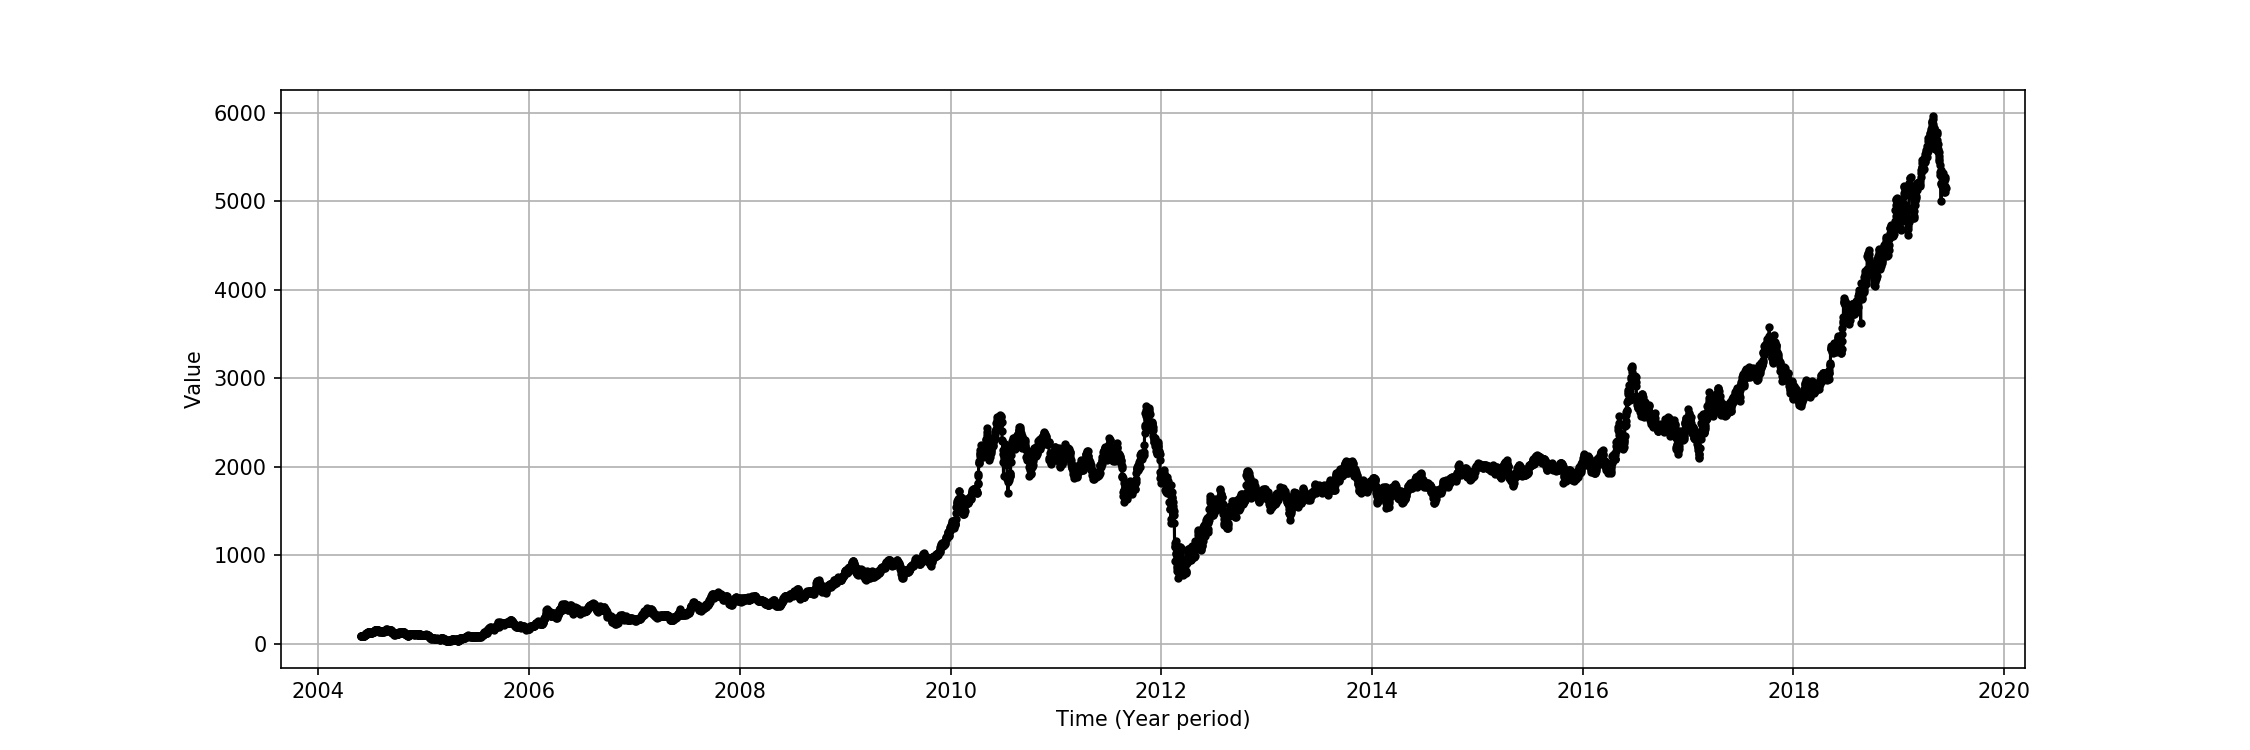
\includegraphics[width=\linewidth]{source_ts_LKOH.png}
		\caption{\label{fig:fig1} Цена акции Лукойл}
	\end{figure}
	Преобразовав временной ряд с помощью следующей формулы:
	\begin{equation}
		y_t = \ln(y_t / y_{t-1})
	\end{equation}
	\begin{figure}[H]
		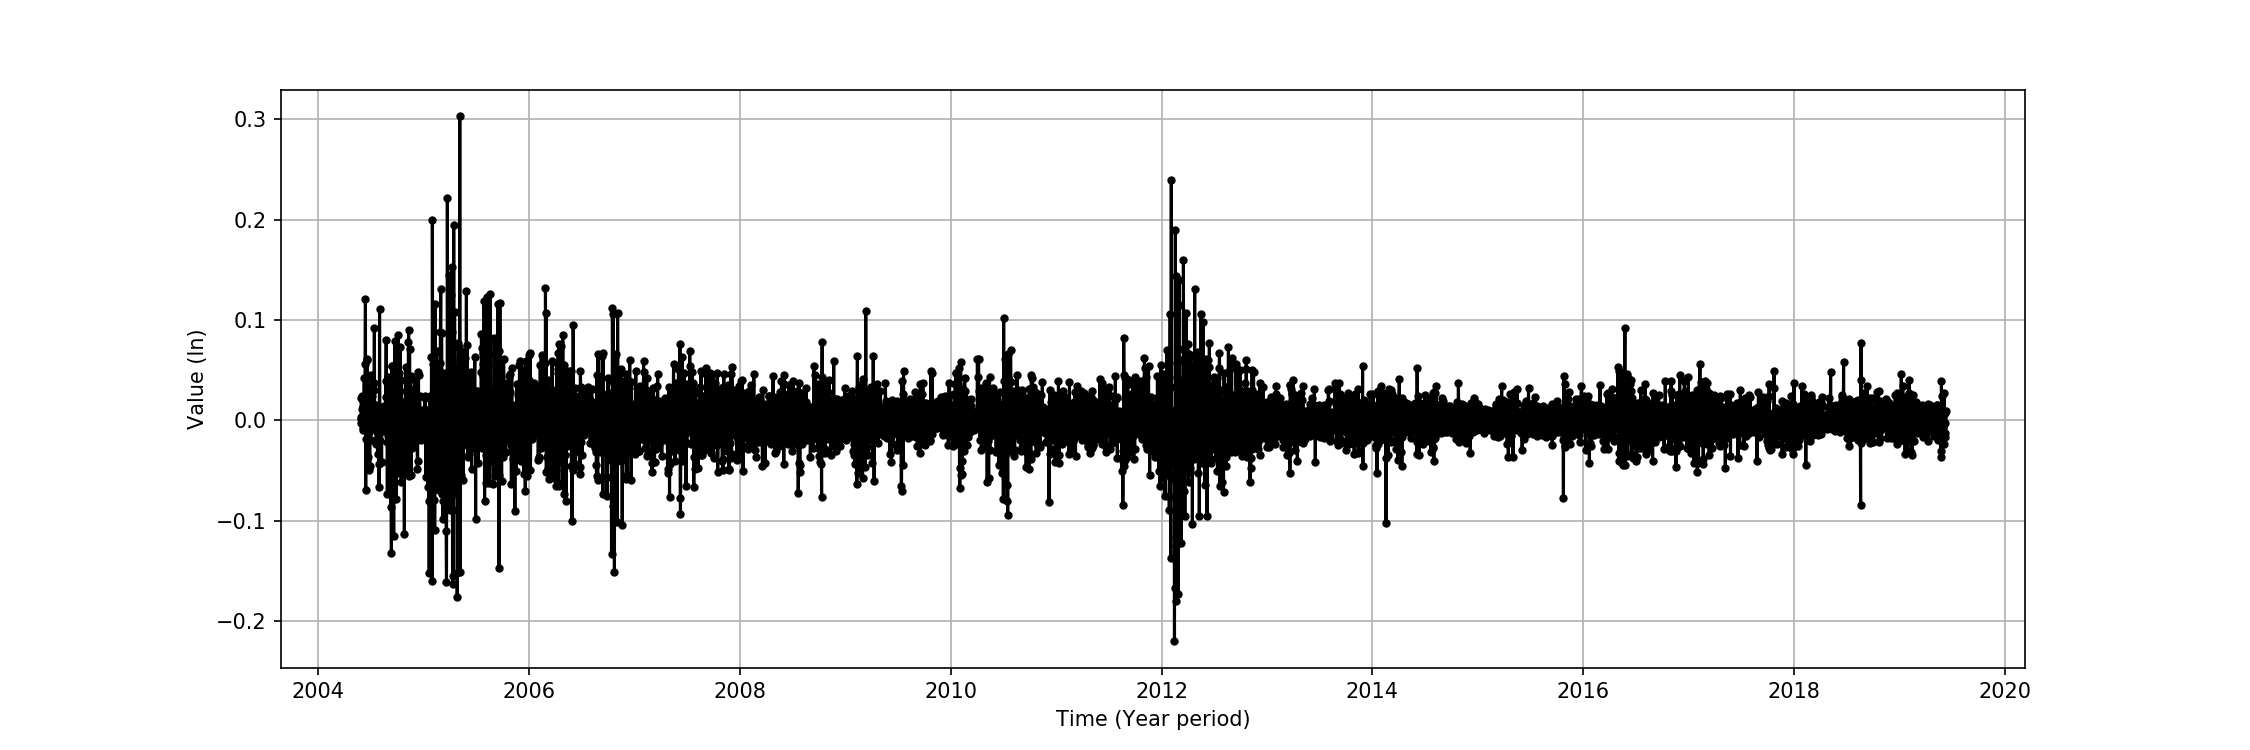
\includegraphics[width=\linewidth]{source_ln_ts_LKOH.png}
		\caption{\label{fig:fig2} Натуральный логарифм отношения цены во времени с лагом 1}
	\end{figure}
	В результате применения ICSS процедуры (которая использует KL-CUSUM метод обнаружения сдвигов) было получено 3 возможных сдвига временного ряда:
	\begin{enumerate}
		\item 2006-11-16 - Заявление Лукойл об увеличении количества выпускаемого топлива (бензин) на 23\%
		\item 2011-12-22 - Вступают в силу поправки Налогового Кодекса, согласно которым акциз на топливо увеличиться. Так же публикация результатов финансового года для компании (по данным отчётов прибыль выросла на 15\%)
		\item 2012-11-12 - Снижение экспорта нефтепродуктов через терминалы ЛУКОЙЛ (до 20\%)
	\end{enumerate}
	\begin{figure}[H]
		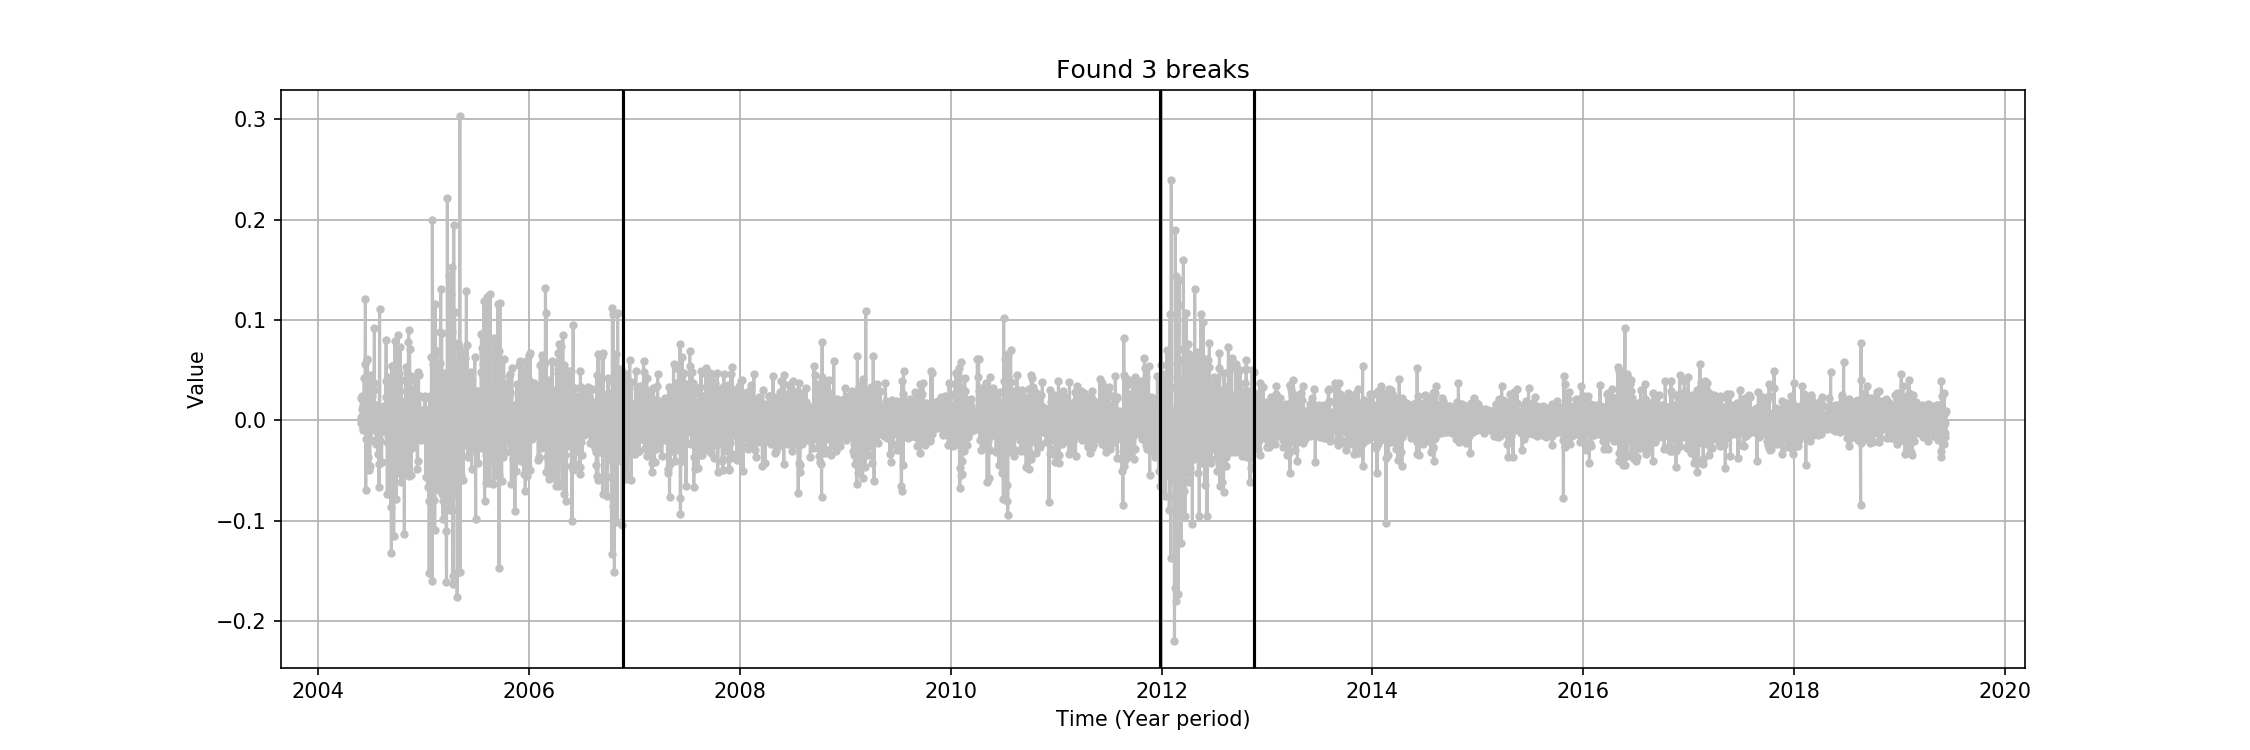
\includegraphics[width=\linewidth]{ru_stock_simulation_LKOH.png}
		\caption{\label{fig:fig3} Структурные сдвиги временного ряда}
	\end{figure}
	Важно заметить, что ICSS алгоритм (KL-CUSUM) может быть улучшен для получения более точных результатов. В этом случае необходимо вести исследования в следующих направлениях:
	\begin{enumerate}
		\item Апробация методов IT, LTM с сочетании с ICSS процедурой
		\item Улучшении возможностей ICCS процедуру такие как ML-KL-ICSS
	\end{enumerate}

\end{document}
